\begin{frame}
\begin{itemize}
\item Large text collections often require topic triage quickly in low-resource settings (e.g. natural disaster, political instability). \pause
\item Analysts need to examine multilingual text collections, but are scarce in one or more languages.
\end{itemize}
\end{frame}

\begin{frame}{Modeling Multilingual Topics}
\begin{figure}
\begin{center}
\begin{overprint}
\onslide<1>\centerline{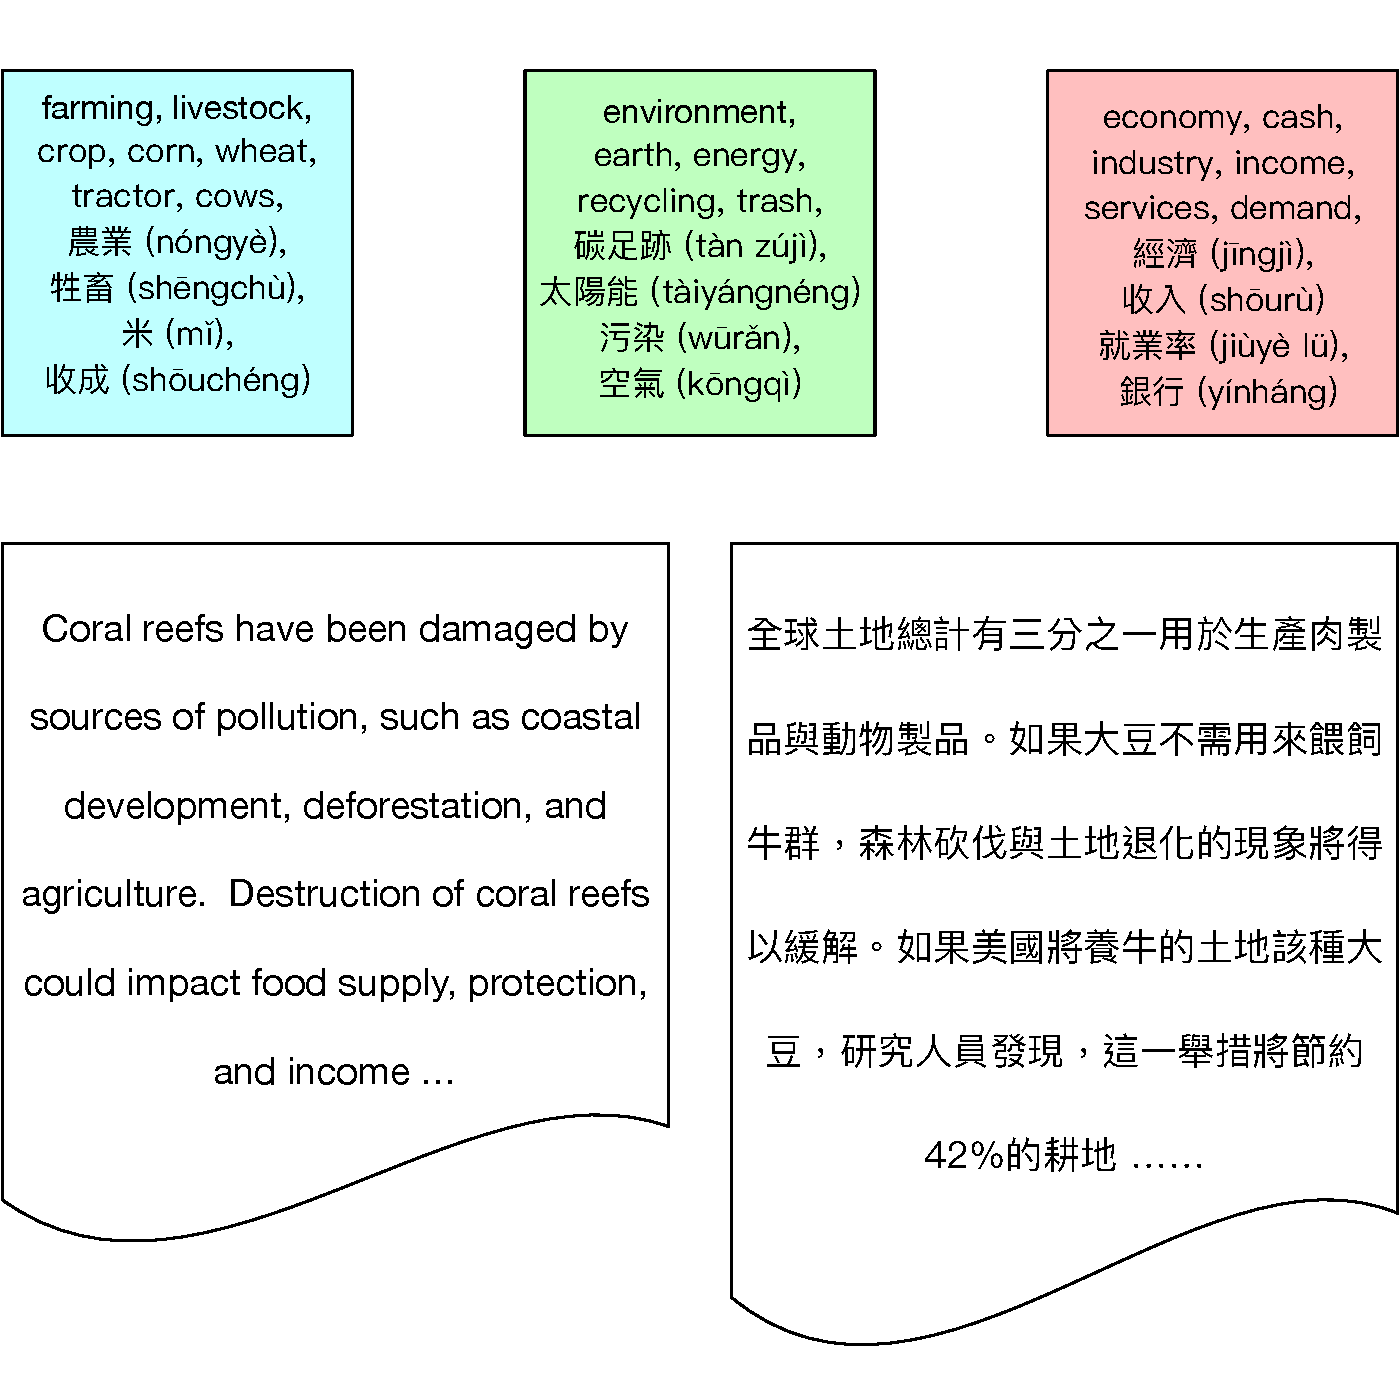
\includegraphics[width=0.7\textwidth]{articles1.pdf}}
\onslide<2>\centerline{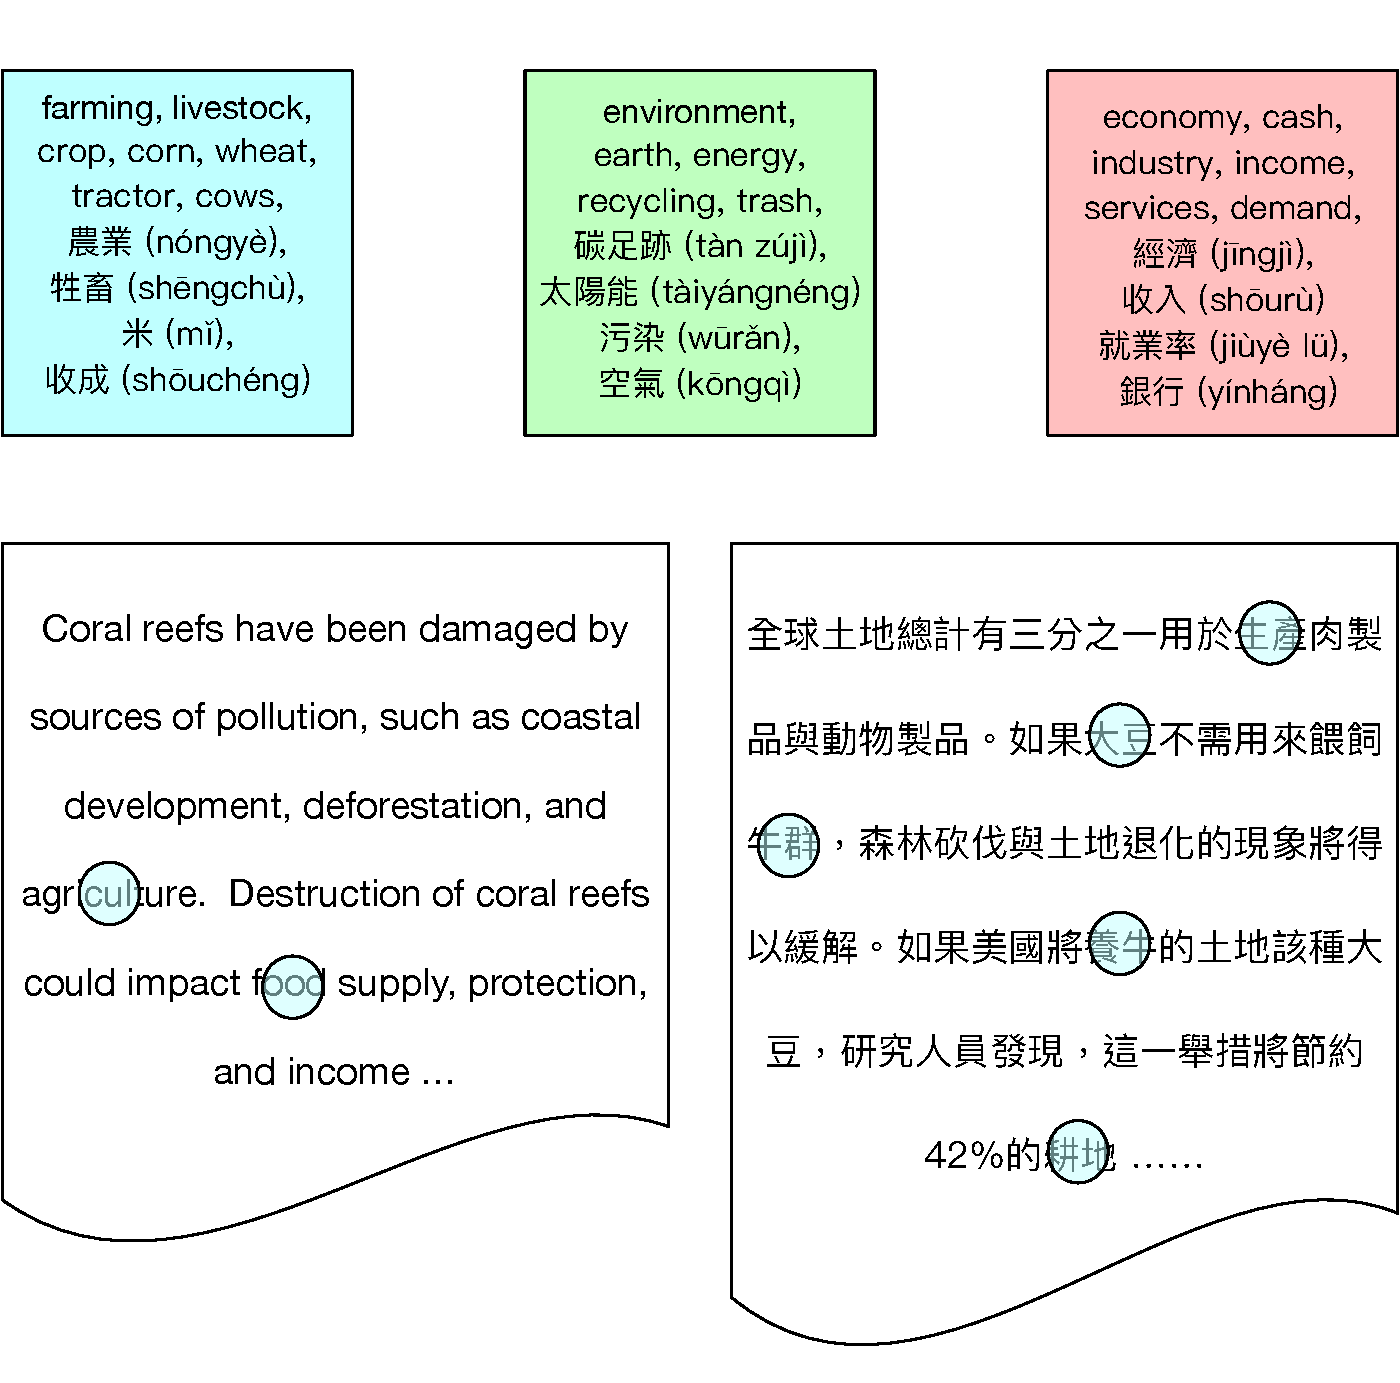
\includegraphics[width=0.7\textwidth]{articles2.pdf}}
\onslide<3>\centerline{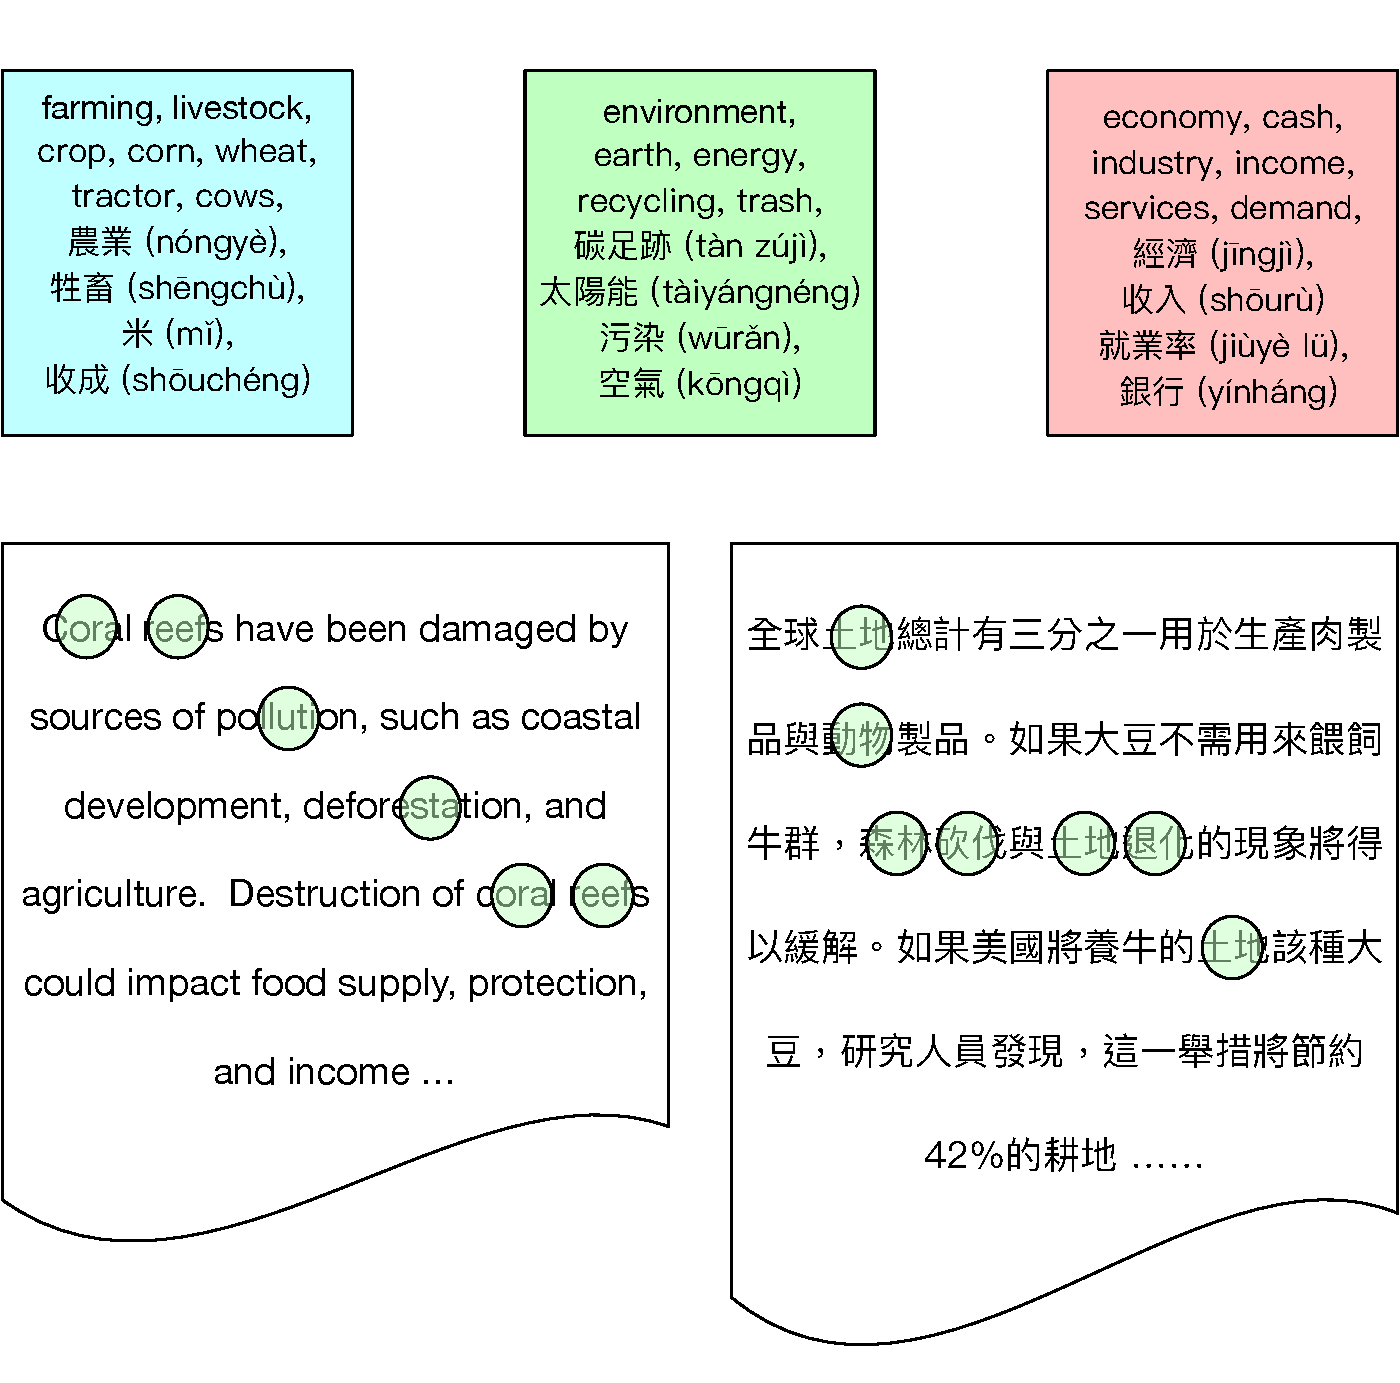
\includegraphics[width=0.7\textwidth]{articles3.pdf}}
\onslide<4>\centerline{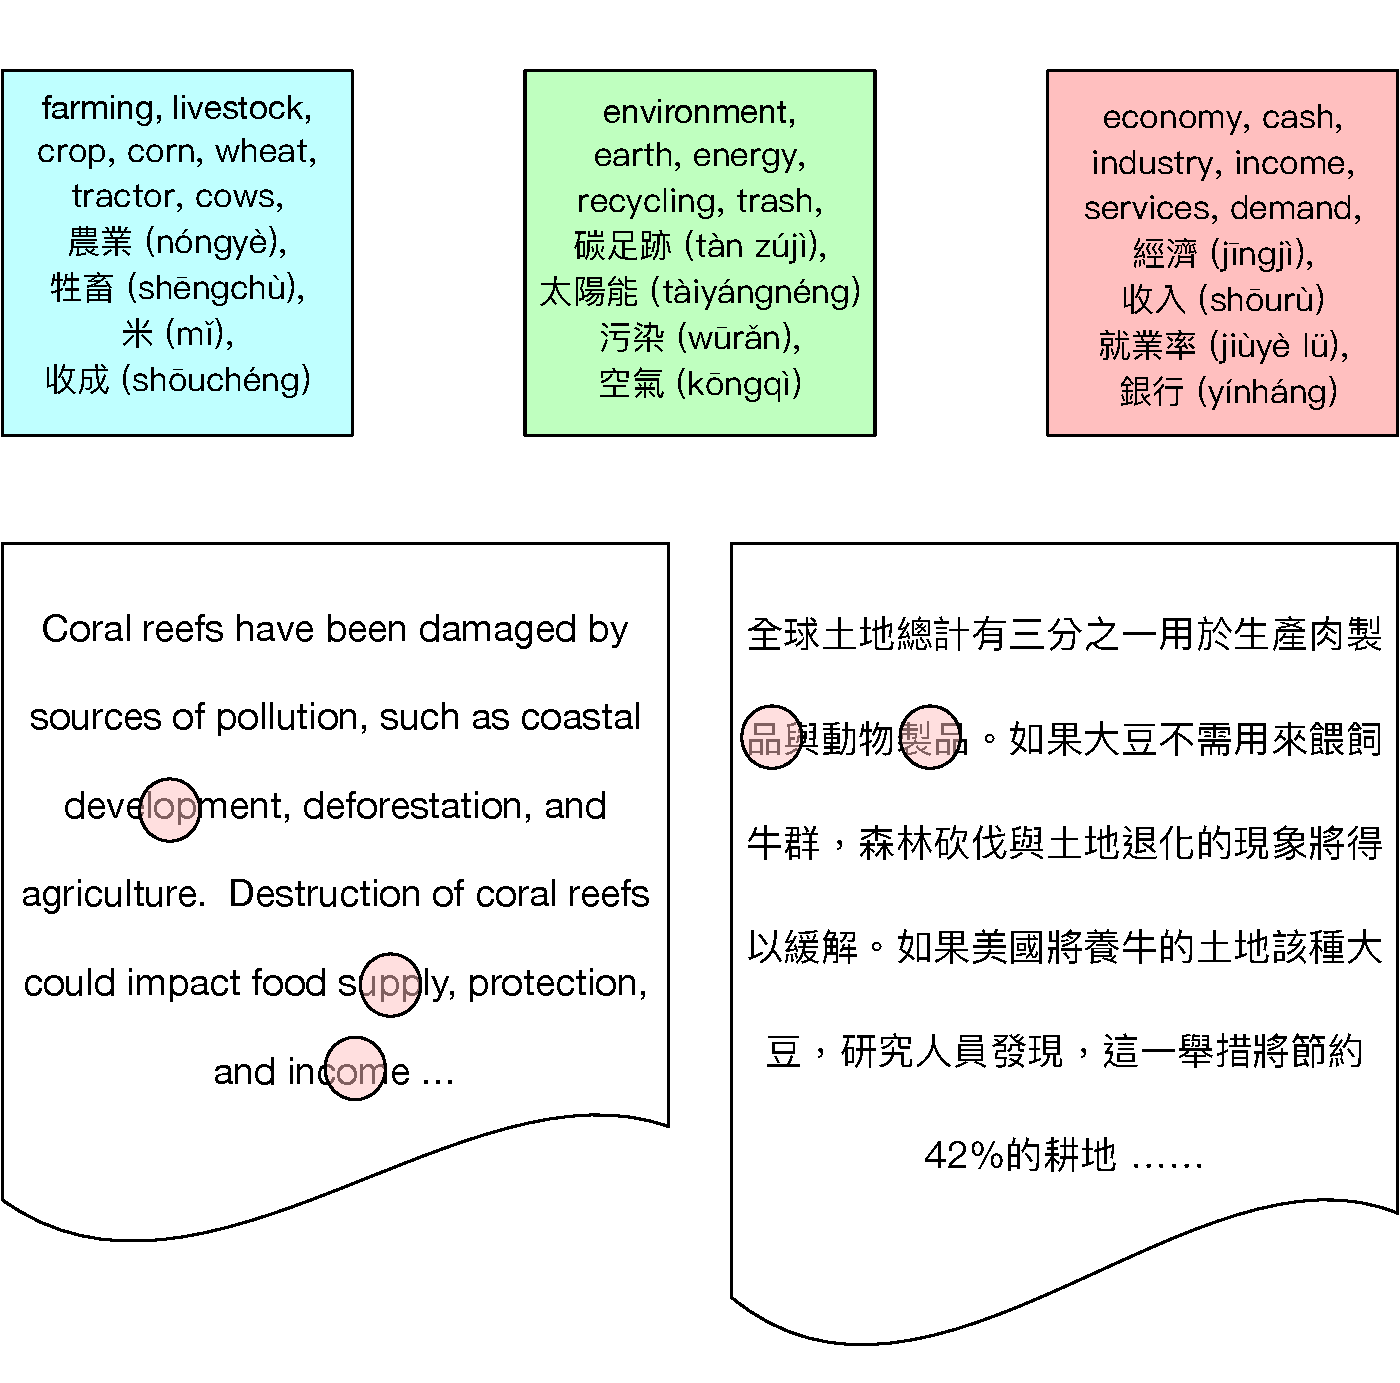
\includegraphics[width=0.7\textwidth]{articles4.pdf}}
\onslide<5->\centerline{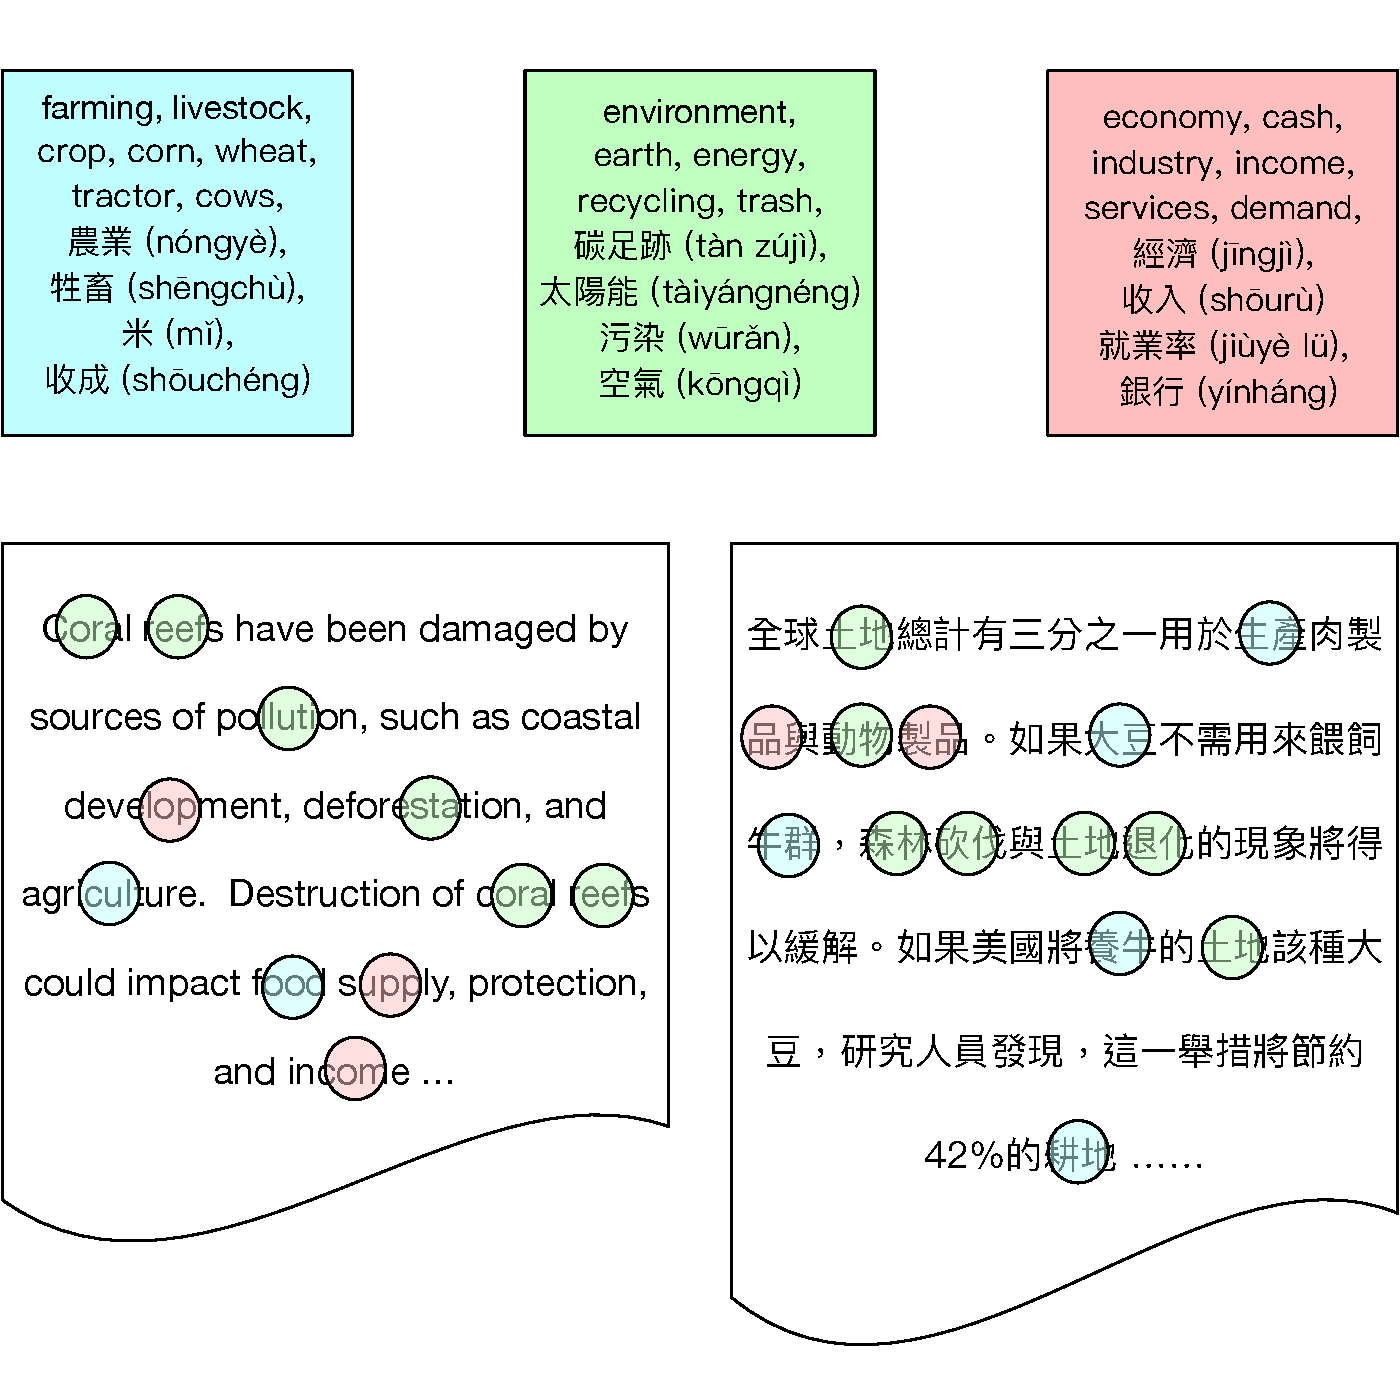
\includegraphics[width=0.7\textwidth]{articles5.pdf}}
\end{overprint}
\end{center}
\end{figure}
\end{frame}

\begin{frame}{Generative Approaches}
\begin{itemize}
\item Polylingual Topic Model~\citep{mimno-2009}
\item Joint\abr{lda}~\citep{jagarlamudi-2010}
\item Polylingual Tree-based Topic model~\citep{hu-2014-ptlda} 
\item \abr{mcta}~\citep{shi-2016} \pause
\vspace{1cm}
\end{itemize}
\textbf{These methods are slow, assume extensive knowledge about languages, and preclude human refinement.}
\end{frame}


